\ifgerman{\chapter{Auswertung}}{\chapter{Implementation}}
\label{sec:implementation}

\section{Simulation Environment}

\todo{finken parameter estimation}

\todo{controller tuning}

\todo{simulation parameters}

\todo{script structure}


\section{Communication V-REP - Quadrocopters}
\label{sec:commImplementation}

This chapter describes the implementation of the requirements on the Java-API, which ware discussed in \ref{sec:communication} of \ref{chap:theo}. It begins with an overview of the software architecture and continues with the explanation of the created projects, classes and their use. It helps understanding how the communication between the V-REP and the quadrocopters is implemented and how to use the API or extend it in order to implement other mixed-reality scenarios.\\
Note that this is just a brief explanation of the Java-API implementation. If you want to go in details refer to the Javadoc which is also provided as an attachment to this paper.

\subsection{Software architecture}

add description of software architecture here.


\begin{figure}[h!]
 \begin{center}
  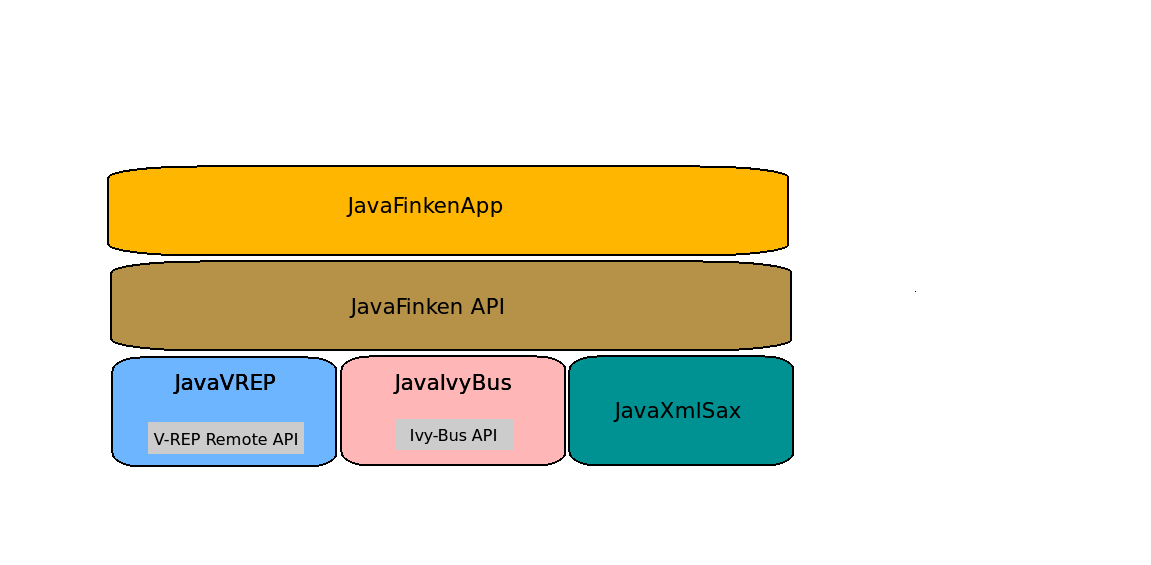
\includegraphics[scale=0.6]{apiArchitecture.png}
 \end{center}
  \caption{Java-API architecture\label{fig:apiArchitecture}}
\end{figure}

\subsection{V-REP RemoteAPI requirements implementation}
\label{sec:vrepImplementation}

All the functionality, that deals with the V-REP and was discussed in \ref{sec:requirementsVREP} of \ref{chap:theo} is implemented as a single Java project called \textit{JavaVREP}.\\
 The project uses the V-REP Remote-API Java binding - package \textit{coppelia} (containing 12 Java classes) and the \textit{libremoteApiJava.so} or \textit{libremoteApiJava.dll} (depending if the platform is Linux or Windows). The \textit{libremoteApiJava.so} should be placed in the Java home directory, e.g \textit{/usr/lib/jvm/java-8-oracle/jre/lib/amd64}, in order for the project to be compiled.\\
The main class is the \textit{VrepConnection.java}, which is a wrapper of the \textit{remoteApi.java} class provided by the V-REP remote API. Its singleton instance can be retrieved by calling:

\begin{center}
\begin{tabular}{c}
\begin{lstlisting}[basicstyle=\small]
VrepConnection connection = VrepConnectionUtils.getConnection();
\end{lstlisting}
\end{tabular}
\end{center}

The above expression loads the remote API library and returns the instance of \textit{VrepConnection} on which the Remote API functions are called. For example to retrieve all objects in a scene the following function have to be called on the \textit{VrepConnection} instance:

\begin{center}
\begin{tabular}{c}
\begin{lstlisting}[basicstyle=\small]

connection.simxGetObjects();

\end{lstlisting}
\end{tabular}
\end{center}

The interfaces \textit{VrepServer} and \textit{VrepClient} and their implementations \textit{StandardVrepServer} and \textit{StandardVrepClient} describe the two end-points of the communication. The \textit{VrepServer} describes the IP address and the port number of the machine on which the V-REP is running. In order to connect to a V-REP server we have to create in instance of the \textit{VrepServer} and open the client:

\begin{center}
\begin{tabular}{c}
\begin{lstlisting}[basicstyle=\small]
VrepConnection connection;
VrepClient     client;
VrepServer     server;

connection = VrepConnectionUtils.getConnection();
client     = VrepClientUtils.getClient();
server     = new StandardVrepServer("127.0.0.1", "19999");

if (server.isFree()) {
// already opened a server on this IP and port.
}

client.connectToServer(server);

if (!client.isConnected()) {
// error in connection
} 
\end{lstlisting}
\end{tabular}
\end{center}

The above example shows how to connect to a V-REP server 




\section{\todo{fancy name }}

\section{Quadcopter}



% example for bar plots
%\begin{tikzpicture}
%  \centering
%  \begin{axis}[
%        ybar = 0,
%    height=6cm,
%    width=15cm,
%    enlarge x limits={rel=0.1},
%    axis lines*=left,
%    ymin=0,
%    ymax=50,
%     legend style={at={(0.5,-0.27)},
%        anchor=north,legend columns=-1},
%        ylabel={\#Anzahl Blöcke},
%        xlabel={Halstead Volumen},
%        cycle list = {black,black!70,black!40,black!10},
%        symbolic x coords={10,20,30,40,50,70,90,120,300,750,>750},
%     xtick=data,
%        nodes near coords,
%    every node near coord/.append style={
%        anchor=mid west,
%        rotate=90 }]
%     \addplot+[] coordinates {(10,3) (20,18) (30,8)(40,1)(50,0)(70,6)(90,6)(120,0)(300,2)(750,0)(>750,0)};
%    \addplot+[fill,text=black] coordinates {(10,3) (20,28) (30,22)(40,7)(50,2)(70,4)(90,11)(120,1)(300,1)(750,2)(>750,0)};
%   \addplot+[fill,,text=black] coordinates {(10,1) (20,1) (30,17)(40,30)(50,10)(70,17)(90,10)(120,8)(300,5)(750,1)(>750,0)};
%    \legend{Modell1,Modell2,Modell3}
%  \end{axis}
%\end{tikzpicture}
%
%
%
%\begin{tikzpicture}
%  \centering
%  \begin{axis}[
%        ybar = 0,
%    height=6cm,
%    width=15cm,
%    enlarge x limits={rel=0.1},
%    axis lines*=left,
%    ymin=0,
%    ymax=70,
%     legend style={at={(0.5,-0.27)},
%        anchor=north,legend columns=-1},
%        ylabel={\#Anzahl Blöcke},
%        xlabel={Anzahl Elemente pro Block},
%        cycle list = {black,black!70,black!40,black!10},
%        symbolic x coords={10,20,30,40,50,70,90,120,300,750,>750},
%     xtick=data,
%        nodes near coords,
%    every node near coord/.append style={
%        anchor=mid west,
%        rotate=90 }]
%     \addplot+[] coordinates {(10,29) (20,6) (30,3)(40,4)(50,0)(70,0)(90,0)(120,0)(300,2)(750,0)(>750,0)};
%    \addplot+[fill,text=black]  coordinates {(10,56) (20,11) (30,4)(40,1)(50,3)(70,3)(90,0)(120,1)(300,0)(750,2)(>750,0)};
%    \addplot+[fill,,text=black] coordinates {(10,41) (20,25) (30,10)(40,7)(50,7)(70,2)(90,2)(120,1)(300,3)(750,2)(>750,2)};
%    \legend{Modell1,Modell2,Modell3}
%  \end{axis}
%\end{tikzpicture}

